\chapter{Introduction}
\label{chap:intro}

%%%%%%%%%%%%%%%%%%%%%%%%%%%%%%%%%%%%%%%%%%%%%%%%%%%%%%%%%%%%%%%%%%%%%%%%%%%%%%%
\section{Background}
\label{sec:chap1-background}

%Intro paragraph\\
%-talk about the increasingly important role of simulation in nuclear?\\
%-challenges for today's nuclear fleet which simulation is well-poised to tackle\\
%-segue into talk about nuclear reactor / neutron physics paragraph\\
%-important to have predictive simulation - needs to be able to extrapolate\\
%-based on empirical models\\
%-complicated core designs, such as the AP1000\\
%-really need to motivate complicated designs since this is relevant to my work\\
%-set the stage for why full-core predictive simulation is needed!!!\\
%-perhaps this is more detail than is necessary for background?\\
%-need to account for angular dependence of neutron flux (e.g. "transport" methods)\\

Physics simulation has long played an important role in nuclear reactor physics and engineering. The nuclear industry relies on computational modeling of the neutron physics in reactors to predict core reactivity, power distributions, fuel depletion, transient behavior, etc. to ensure the safety and reliability of the current fleet of \ac{LWRs}. Predictive simulations are necessary to evaluate innovations which seek to improve the reactor safety and fuel cycle economics, such as reduced safety margin uncertainties, high-burnup fuels, and extended cycle lengths. In addition, simulation is used to assess the technical competencies of advanced reactor technologies such as Small Modular Reactors (SMRs), Sodium Fast Reactors (SFRS), Molten Salt Reactors (MSRs), High Temperature Gas Reactors (HTGRs), among other possible designs. 

Many Generation III+ reactor designs, such as the Westinghouse AP1000 \ac{PWR}, optimize performance with complicated core designs. A variety of reactivity control mechanisms -- including partially-inserted control rods, ``grey'' control poisons, \ac{IFBA}, soluble boron, etc. -- along with axial enrichment zoning are used to improve performance metrics such as power peaking factors. The reactor analysis methods in widespread use today assume a ``smoothly'' varying flux distribution, and are not well-suited to model highly localized flux gradients which result from these complex core configurations. New high-fidelity simulation tools are needed to accurately capture neutron physics in enable advanced reactor designs.

The nuclear reactor physics community has long strived for whole-core transport based tools for nuclear reactor analysis. Transport-based methods would enable more accurate core power distributions to be calculated without the approximations needed for today’s tools based upon diffusion theory. Although the computational requirements for full-core transport-based simulations have precluded their widespread development, the continuing growth of cheap parallel processing power has made the prospects for such tools increasingly feasible.


First paragraph\\
-wish to replace diffusion with full-core transport\\
-benefits of improved reactor analysis tools\\
-HPC may make this possible\\

Second paragraph\\
-compare contrast competing algorithms - Monte Carlo and deterministic transport\\
-tradeoff between computational speed/efficiency and accuracy\\
-crux of deterministic methods are MGXS\\

Third paragraph\\
-MGXS generation tools developed for coarse mesh diffusion\\
-Existing codes/techniques may not be adequate for full-core transport\\
-to take full advantage of full-core transport methods, need MGXS of appropriate accuracy\\
-must quantify approximation errors in MGXS for full-core transport \\
-brief overview of MGXS approximations\\
-specifically pinpoint angular-dependence and spatial self-shielding\\

Fourth paragraph\\
-outline following sections\\

-need to mention goal of making fast deterministic transport as accurate as Monte Carlo\\
-should this just be a summary before leading into the following sections???\\


\begin{itemize}
  \item mention advantages of full core transport
  \begin{itemize}
    \item optimize core design
    \item analyze accident-tolerant fuels
    \item reduce uncertainty magins on CHF
    \item analysis of advanced non-LWR designs
  \end{itemize}
\end{itemize}

\begin{itemize}[noitemsep]
  \item mention two pronged approach - quantify MGXS approximations and apply clustering
  \item provide motivation for need for new approaches for full-core transport
\end{itemize}

\begin{figure}
\begin{subfigure}{.5\textwidth}
  \centering
  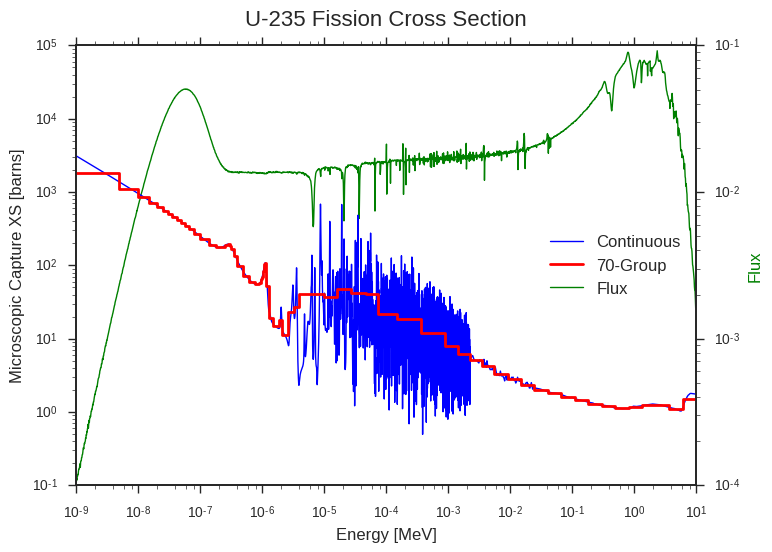
\includegraphics[width=\linewidth]{figures/intro/u235-fission-70}
  \caption{}
  \label{fig:assm-cells}
\end{subfigure}%
\begin{subfigure}{.5\textwidth}
  \centering
  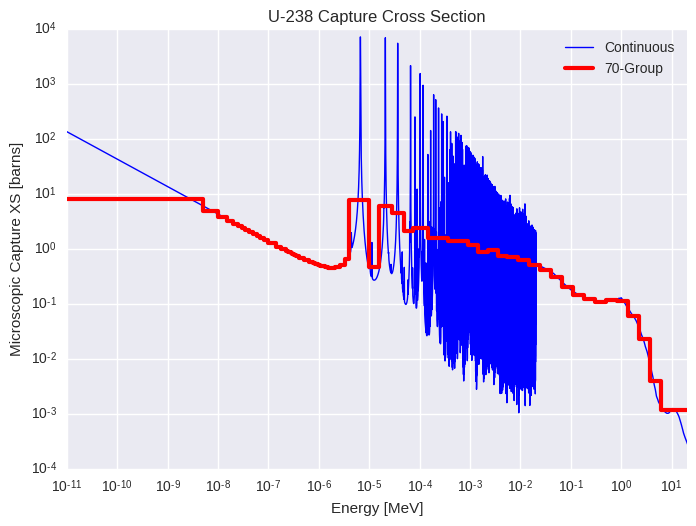
\includegraphics[width=\linewidth]{figures/intro/u238-capture-70}
  \caption{}
  \label{fig:colorset-cells}
\end{subfigure}
\begin{subfigure}{.5\textwidth}
  \centering
  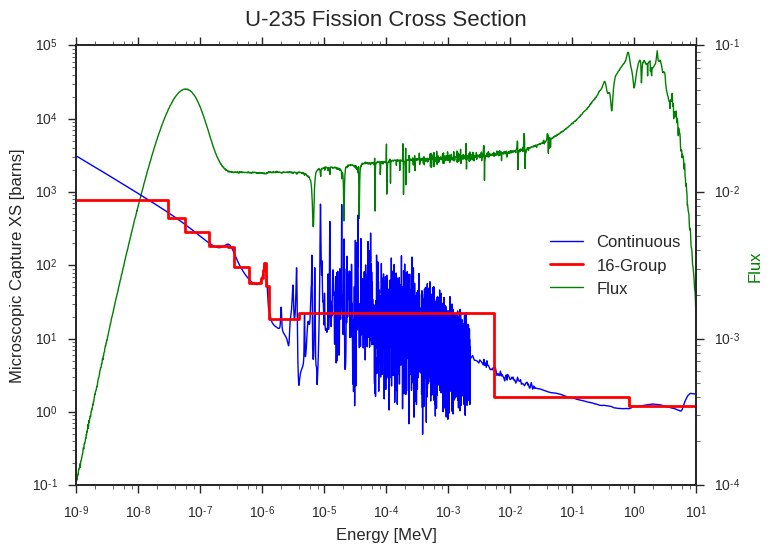
\includegraphics[width=\linewidth]{figures/intro/u235-fission-16}
  \caption{}
  \label{fig:assm-unique-neighbors}
\end{subfigure}
\begin{subfigure}{.5\textwidth}
  \centering
  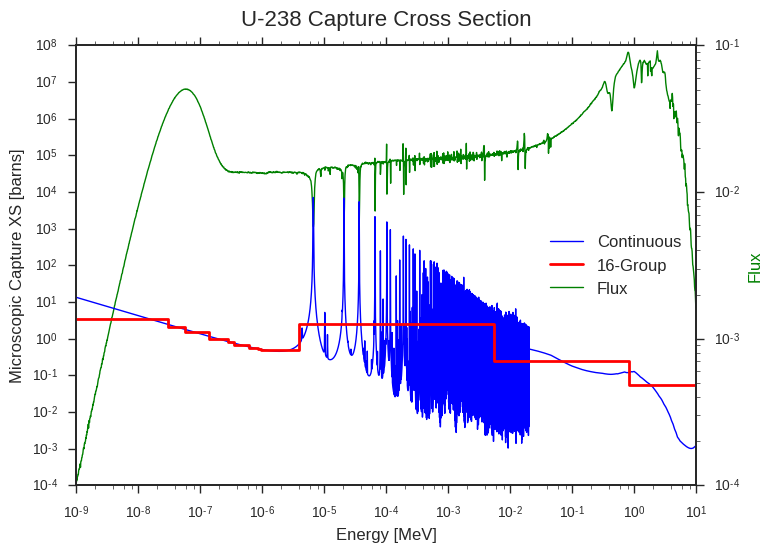
\includegraphics[width=\linewidth]{figures/intro/u238-capture-16}
  \caption{}
  \label{fig:colorset-unique-neighbors}
\end{subfigure}
\begin{subfigure}{.5\textwidth}
  \centering
  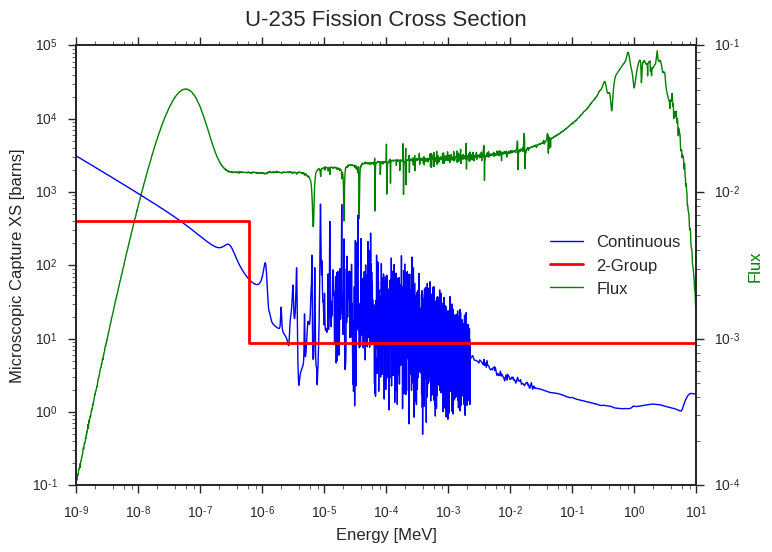
\includegraphics[width=\linewidth]{figures/intro/u235-fission-2}
  \caption{}
  \label{fig:assm-neighbors}
\end{subfigure}
\begin{subfigure}{.5\textwidth}
  \centering
  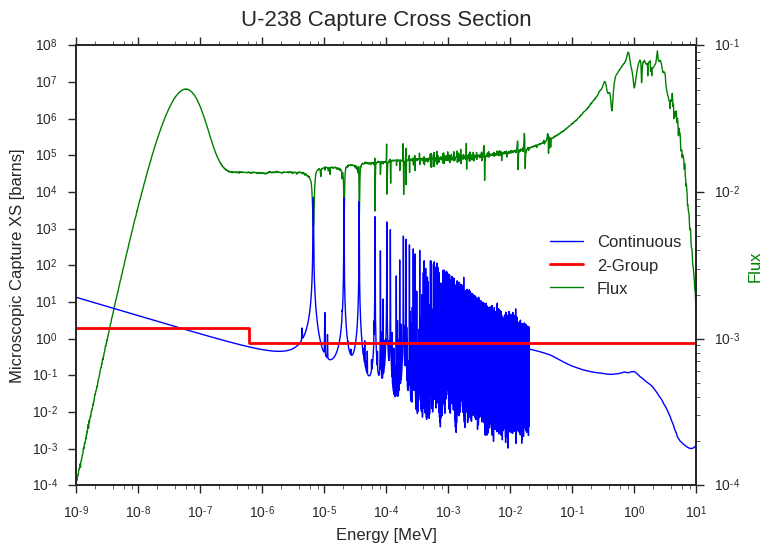
\includegraphics[width=\linewidth]{figures/intro/u238-capture-2}
  \caption{}
  \label{fig:colorset-neighbors}
\end{subfigure}
\caption[Uranium-235 and Uranium-238 cross sections]{Continuous energy and multi-group cross sections for U-235 fission (left) and U-238 capture (right) reactions in a PWR spectrum for 70-, 16- and 2-groups.}
\label{fig:pwr-ce-mg-xs}
\end{figure}


%%%%%%%%%%%%%%%%%%%%%%%%%%%%%%%%%%%%%%%%%%%%%%%%%%%%%%%%%%%%%%%%%%%%%%%%%%%%%%%
\section{High-Performance Computing Trends}
\label{sec:chap1-hpc-trends}

\cite{Hunter_Sutton_2013}


%%%%%%%%%%%%%%%%%%%%%%%%%%%%%%%%%%%%%%%%%%%%%%%%%%%%%%%%%%%%%%%%%%%%%%%%%%%%%%%
\section{Whole-Core Neutron Transport Simulations}
\label{sec:chap1-whole-core-transport}

\begin{dmath}
\label{eqn:chap1-transport-eqn-6d}
\mathbf{\Omega} \cdot \nabla \Psi(\mathbf{r},\mathbf{\Omega},E) + \Sigma^T(\mathbf{r},E)\Psi(\mathbf{r},\mathbf{\Omega},E) = \int_{0}^{\infty} \mathrm{d}E' \int_{4\pi} \mathrm{d}\mathbf{\Omega'}\Sigma^S(\mathbf{r},{\mathbf{\Omega'}\rightarrow\mathbf{\Omega}},{E'\rightarrow E}) \Psi(\mathbf{r},\mathbf{\Omega'},E') + \frac{\chi(\mathbf{r},E)}{4\pi k_{eff}} \int_{0}^{\infty} \mathrm{d}E' \nu\Sigma^F(\mathbf{r},E') \int_{4\pi} \mathrm{d}\mathbf{\Omega'}\Psi(\mathbf{r},\mathbf{\Omega'},E')
\end{dmath}

Each of the variables in use is defined in \autoref{tab:moc-variables}. This is a balance equation between neutrons lost to transport, lost to absorption, produced or lost from scattering and those produced from fission. It should be noted that this equation assumes isotropic emission from fission.

\begin{table}[hbt]
  \caption{Variables in the Boltzmann equation.}
  \label{tab:chap1-variables}
  \begin{center}
    \begin{tabular}{ l l }
    \toprule
    Variable & Description \\
    \midrule
    $\mathbf{r}$ & Spatial position vector \\
    $\mathbf{\Omega}$ & Angular direction vector \\
    $E$ & Neutron energy \\
    $\Psi$ & Angular neutron flux \\
    $k_{eff}$ & Effective neutron multiplication factor \\
    $\Sigma^T$ & Neutron total cross-section \\
    $\Sigma^S$ & Neutron scattering cross-section \\
    $\Sigma^F$ & Neutron fission cross-section \\
    $\chi$ & Energy spectrum for fission neutrons \\
    $\nu$ & Average number of neutrons emitted per fission \\
    \bottomrule
  \end{tabular}
  \end{center}
\end{table}


%%%%%%%%%%%%%%%%%%%%%%%%%%%%%%%%
\subsection{Monte Carlo Methods}
\label{subsec:chap1-monte-carlo}


%%%%%%%%%%%%%%%%%%%%%%%%%%%%%%%%%%
\subsection{Deterministic Methods}
\label{subsec:chap1-deterministic}

\begin{itemize}
  \item 2D/1D methods in MPACT, nTracer
  \item Denovo, PDT, 3D OpenMOC, etc.
\end{itemize}


%%%%%%%%%%%%%%%%%%%%%%%%%%%%%%%%%%%%%%%%%%%%%%%%%%%%%%%%%%%%%%%%%%%%%%%%%%%%%%%
\section{Multi-Group Cross Sections}
\label{sec:chap1-mgxs}

\begin{itemize}[noitemsep]
  \item black magic ``crux'' of deterministic methods
  \item need accurate \ac{MGXS} for whole core transport methods
  \item motivate \ac{MC} for \ac{MGXS}
\end{itemize}